%%%%%%%%%%%%%%%%%%%%%%%%%%%%%%%%%%%%%%%%%%%%%%%%%%%%%%%%%%%%%%%%%%%%%%%%%%%%%%
% Detta är ett exempel på fancyhdr.
%
% För mer information, använd xdvi för att titta på filen:
% /usr/local/lib/texmf/doc/latex/fancyhdr/fancyhdr.dvi
%%%%%%%%%%%%%%%%%%%%%%%%%%%%%%%%%%%%%%%%%%%%%%%%%%%%%%%%%%%%%%%%%%%%%%%%%%%%%%


\documentclass[11pt]{article}

\usepackage[utf8]{inputenc}
\usepackage[T1]{fontenc}                              % För svenska bokstäver
\usepackage[swedish]{babel}             % För svensk avstavning och svenska o rubriker (t ex "innehåll)
\usepackage{fancyhdr}
\usepackage{enumitem} % resume numbering in enumerations
\usepackage[bottom = 110pt]{geometry} % to change the page dimensions
\usepackage{graphicx} % support the \includegraphics command and options
\usepackage[parfill]{parskip} % Begin paragraphs with an empty line rather than an indent
\usepackage{verbatim} % adds environment for commenting out blocks of text & for better verbatim
\pagestyle{fancy} % options: empty , plain , fancy
\usepackage{hyperref} % href
\usepackage{nameref} % Enable referring to the actual name of the chapter
\usepackage[backend=biber,sorting=none]{biblatex}
%\bibliography{references.bib}
\usepackage{url}
\usepackage{fancyvrb}
\usepackage{graphicx}
\usepackage{caption}
\usepackage{subcaption}



\title{Mobile-first eller Desktop-first, en studie om weblösningar till responsiva web design}
\author{Eduardo Castaneda}           
% \date Blir dagens datum om det utelämnas

\pagestyle{fancy}               % Fräcka sidhuvuden
\addtolength{\headwidth}{0cm}   % Sidhuvd bredare än texten.


% Följande kommandon definerar vad som ska finnas i sidhuvud och
% sidfot. Om man skriver dubbelsidiga dokument anger man två alternativ
% med komma mellan. Den första gäller då för udda sidor och den andra
% för jämna sidor. Bokstäverna ska tolkas som:
% L = left, C = center, R = right,
% E = even (jämna sidor), O = odd (udda sidor)
% E och O fyller ingen funktion om man inte har optionen twopage definierad

%\fancyhead[L]{\texttt{\leftmark}}	% Vänstertext i sidhuvud
%\fancyhead[R]{\bfseries\rightmark}	% Högertext i sidhuvud
%\fancyfoot[C]{- sida \thepage\ -}	% Mittentext i sidfot
%\fancyfoot[LO,RE]{Eduardo Castaneda}		% Vänster udda, höger jämna sidor
%\fancyfoot[LE,RO]{Informationsteknologi}	% Vänster jämna, höger udda sidor
\renewcommand{\headrulewidth}{0.4pt}
\renewcommand{\footrulewidth}{0.4pt}




\begin{document}

\maketitle                  % Skriver ut rubriken som vi
                                % deklarerade ovan med \title, \author
                                % och eventuellt \date

\newpage

\tableofcontents
\newpage



\section{Bakgrund}

Mobilutvecklingen har under de senaste åren gått fort framåt, vilket har lett till att mobiler numera utvecklas till att fungera likt en handburen minidator. Huvudsyftet med mobiler är inte längre att bara kunna kommunicera med andra, utan även att bland annat ha möjligheten att få ut information genom webben. Att en websida inte längre endast ses i en skrivbordsskärm har gjort att nya webblösningar krävs. En utvecklare måste ha i åtanke att webbdesignen bör fungera för en användare som sitter på kontoret och läser sidan från en skrivbordsskärm, likaväl för en användare som sitter på tåget och läser sidan från mobilen. Responsive web design är en lösning vilken beroende på skärmstorlek renderar samma sida på olika sätt. I responsive web design har det fokuserats på två olika metoder, Mobile-first och Desktop-first. Metoderna grundar sig på att utveckling sker för en typ av skärm först för att sedan utifrån det utveckla så att den sidan även passar för andra skärmar. Det finns mycket kunskap om metoderna var för sig, men inget underlag för valet av metod i olika situationer och inom olika områden. Mobilanvändarna ökar för varje dag medan skrivbordsanvändare minskar med en liten mängd, det största antalet använder sig utav båda, vilket kräver kunskap om när metoderna appliceras bäst för att få effektivare lösningar inom webutveckling.

\subsection{Mobil användare}

Sedan 2007 då Apple visade upp den första versionen av iPhone har utvecklingen för smartphones eskalerat markant. Smartphones ger dig möjligheten att utföra datorliknande handlingar som att få ut information från webben och använda nätbaserade applikationer. Tidigare mobiler har delvis haft den funktionen men fokus har varit mestadels på musikspelare och kamera, då surfande gick trögt och var icke användarvänlig.
Med smartphones, vilket innebar större pekskärmar, gjorde åtkomsten till internet på mobilen mer användarvänlig och har under de senaste åren utvecklats till en oundviklig funktion i dagens mobiler.


Dagens användare av mobiler sträcker sig mellan 15-79 år gamla, av dessa är det cirka 40 \% som använder sig av mobilt internet, i jämförelse med 2008 har det ökat med över 50 \%. Telefonoperatörer har anpassat sig i den nya marknaden och erbjuder abonnemanger vilka innehåller en fast kostnad för surf på ett 3G nät. Då mobilsurf anses som en nödvändig funktion, sätts även krav hos mobiloperatörer, 3G nätet skall ha hög åtkomlighet och ha en hög hastighet. Effekten av att mobilanvändarnas åtkomst till internet ökar, leder till mobilt internet används mer och äldre tjänster ersätts. En tidning i tunnelbanan är inte alls lika vanligt nu som för fem år sen, tidtabeller vid busshållplatsen spelar är inte lika viktiga som förr och att checka-in inför en flygresa behöver inte nödvändigtvis ske via en check-in disk.


Konkurrensen som finns i dagens mobilmarknad har tvingat ledande företag att skapa mobiler med ny teknik till allt lägre priser. Pris, tillgänglighet och användbarhet har gjort att användning av internet via mobilen i världen närmar sig antalet användare av internet via en dator. Analytiker som förutspådde mobilen till att slå i marknaden har i dagsläget fått det bekräftat och förutspår att användare av mobilt internet i världen kommer att passera antalet användare från av Desktop internet [fotnot 2] i 2014 år. Detta kräver från webbplatser att följa målgruppen användare och anpassa webbsidor utifrån de enheter som webbsidor ses ifrån, vilket är till stor del är från mobilen.

\subsection{Desktop användare}
Att mobil användare ökar för varje dag har till viss del betydelse i minskningen av antalet desktop användare. Men datorer har i dagsläget funktioner som gör det osannolikt för mobiler att helt kunna ersätta datorer, funktioner som kräver att man sitter vid en dator och på så sätt sker informationssökandet i webben via desktop. 

Webbdesignen på en mobil är kompakt och uppfyller den nödvändigaste användbarheten.
På desktop är designen mer informationsrikt, vilket ger en större inblick till websidans innehåll och en mer simpel navigering på webbsidan. Det gör att en användare beroende på komplexitet och säkerhet av handlingen väljer att utföra den via en desktop, än via mobilen. En sådan handling kan t.ex. vara bankärenden eller web shopping. Om bankärendet är en simpel koll av saldo eller överföring mellan egna konton, är mobilen en smidig enhet att använda sig av. Däremot om handlingen innebär att betala räkningar eller överföra stora summor pengar väljer man att utföra det via desktoppen, då det ger en större säkerhet och en mer simpel navigering på websidan. Även web shop faller i samma kategori, då användare väljer att söka information om produkten via mobilen, men väljer sedan att utföra köpet via desktop.[fotnot 1] Detta tyder på att användare av mobilt- eller desktop internet inte är endera, utan är användare utav båda, beroende på situation, miljö och kontext.

Det finns ingen grundlig faktum som tyder på att mobilt internet kommer att ta över all desktop internet användande, endast att de kan bli fler. Därför krävs det att man förstorar vyerna kring webutveckling och lösningar som gynnar både mobil- och desktop användning av internet. För även om mobila användare är fler, så går inte att förbise desktop användare.

\subsection{Responsive web design}

Responsive web design är ett koncept som innebär att gränssnittet på en websida ändras beroende på skärmstorlek, vilket således ger möjligheten att ha olika layout på en och samma websida anpassat efter en enhet. Konceptet definierades av Ethan Marcotte (2010) i en artikel kallat A List Apart, som sedan blev en del av boken ”responsive web design” där teorier och praktiska exempel används för att förklara begreppet. 

Syftet med Responsive Web Design är att kunna rendera olika delar av sidan beroende på skärmstorlek för att ge en optimal vy för den enhet websidan ses från. Om tre element renderas bredvid varandra på en desktop site, så vore det optimala för en mobil site att kunna renderar elementen under varandra och även skala ner de till en rimlig storlek, för att på så sätt undvika att artiklarna försvinner, inte visas helt och hållet eller tar för stor plats på skärmen.

Då endast layouten på sidan ändras behövs inga särskilda versioner för varje enhet, vilket gör det möjligt för en webbutvecklare att på ett enkelt sätt utföra en ändring i en fil, istället för antalet versioner. Däremot krävs en flexibel grundlayout för att responsive web design skall fungera, vilket enligt Ethan görs genom tre grundtekniker, Fluid Grid, Fluid Images och Media Queries.

\subsubsection{Fluid Grid}
På en webbsida kan storleken på element definieras på olika sätt. Ett vanligt sätt att definiera element är med bredd och höjd i pixlar. När det definieras i pixlar betyder det att storleken på elementet är förutbestämd vare sig upplösning eller storlek på skärm. I tidigare skede informerade webbutvecklare i vilken upplösning som renderar sidan på bästa sätt och sedan var upp till användaren att ändra upplösning på skärmen för att få den önskade layouten på sidan. I dagsläget finns många olika skärmar, och många olika alternativ till upplösning vilket gör en förutbestämd storlek inte lika optimalt. 

Fluid Grid är en teknik vilken använder sig procentsatser istället för pixlar. När procentsatser används förstoras eller förminskas elementets storlek relativt till webbläsarfönstrets höjd och bredd, vilket gör att sidan anpassas efter användaren istället för tvärtom. Om ett element skall täcka hela bredden på skärmen, sätts bredden till 100 %, en fjärde del av skärmen, 25 % osv. Ett sätt att räkna ut elementens storlek för att få en Fluid Grid, är att dividera pixlarna på elementet med pixlarna på elementets hållare, detta ger ett resultat i procent vilket gör att elementet anpassar sig beroende på sidans totala bredd.

\subsubsection{Fluid Images}
Fluid Images bygger på samma princip som Fluid Grid, däremot är lösningen mer komplext då det innefattar skalning av bilder. Om en bild skalas på fel sätt leder detta till att bilden ser för utsträckt eller för intryckt ut, men om skalning inte görs, kan en bild i princip ta upp all plats på webbsidan och även försvinna ut i kanterna. Inom responsive web design används Fluid Images, vilket innebär en flexible hållare med en önskad storlek, med en bild anpassad till hållaren.  

Med egenskapen ”max-width:100 \% på bilden“ talar man om för webläsaren att bilden skall skalas efter hållaren men endast till max av den originella storleken på bilden. ”width:100\%” talar om att bilden bara får anpassa sig efter hållaren, samtidigt som den får en normal skalning när storleken på webbläsaren minskar och hållaren krymper. Max i ”max-width” ser till att bilden aldrig blir större än bildens verkliga storlek. Om ”max” inte sätts, finns risk att bilden skalas ut, om det inte är vektor grafiska bilder, vilket gör pixelkanter synliga. Däremot så krävs det oftast att man har en bild som redan från början är av önskad storlek. En för liten bild kommer den inte att förstoras då den som störst kan vara 100 \% av bildens ursprungliga storlek.

\subsubsection{Media Queries}
Fluid Grid och Fluid Images skapar tillsammans en del av en responsiv sida då storleken på elementen i sidan renderas utifrån storleken på skärmen. Minskningen eller förstoringen av elementen fungerar däremot endast till en viss gräns. Är storleken på webläsaren för liten, finns risk att element kommer för nära varandra och skapar konflikt i layouten, vilket gör att element hamnar på felaktiga positioner och ger en vy som designmässigt ser förstörd ut. Blir storleken däremot för stor, finns risk att max-width på bilderna uppnås och stannar i storlek, medan andra element följer förstoringen hos webbläsaren, blir för stora och skapar en osymmetri i layouten. Media Queries är en lösning som tillåter element att ha olika värden beroende på skärmstorlek.

Inom responsive web design är bredden och höjden viktiga egenskaper då de avgör hur mycket av en sida skall synas på webläsarfönstret.  Media queries är anrop som görs i CSS filen, där man kollar antingen höjden och eller bredden för att utföra nödvändiga ändringar i layouten för att upprätthålla en bra design. Tillsammans med Fluid Grid och Fluid Image skapar Media Queries en responsiv web design. 

Vid användning av fluid grid och fluid image sätts egenskaper hos element i procentform, t.ex 50 \%. Med en centrering på element, blir resultatet en ruta i mitten av skärmen som täcker 50 \% och har 25 \% utrymme på var sida. När webläsarfönstret minskas till storleken på en mobilskärm, anpassas elementet utifrån skärmen, eftersom fluid grid tekniken används för bredden.

\vspace{0.5cm}
\begin{figure}[h]
\centerline{%
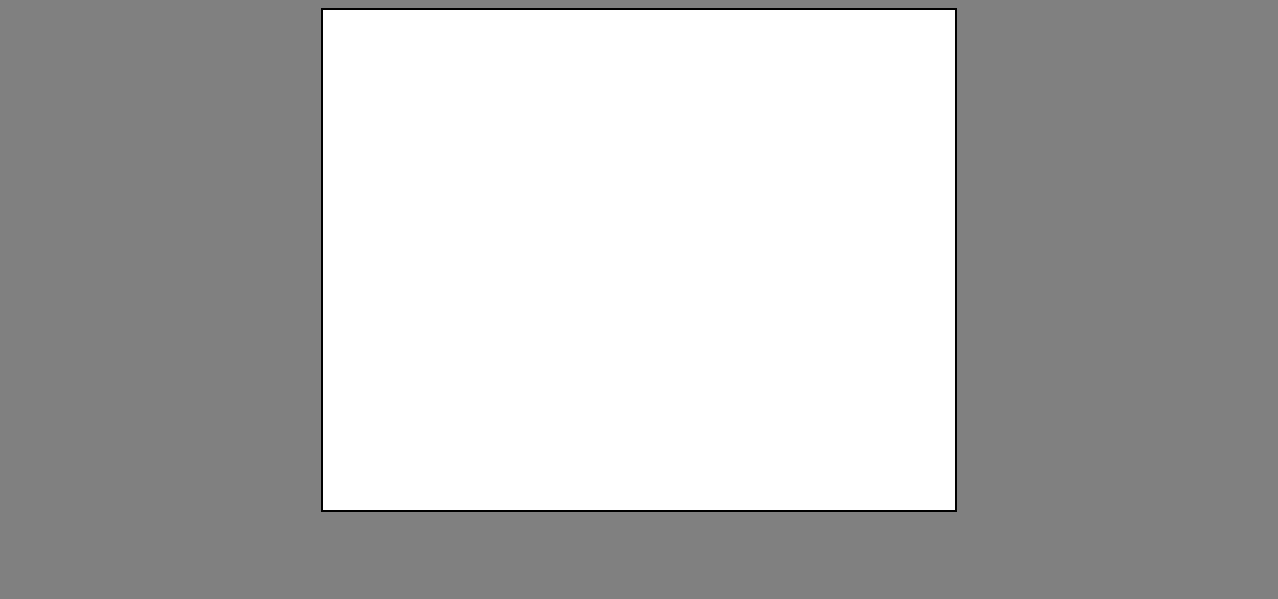
\includegraphics[scale=0.23]{pics/big.png}\hspace{5em}%
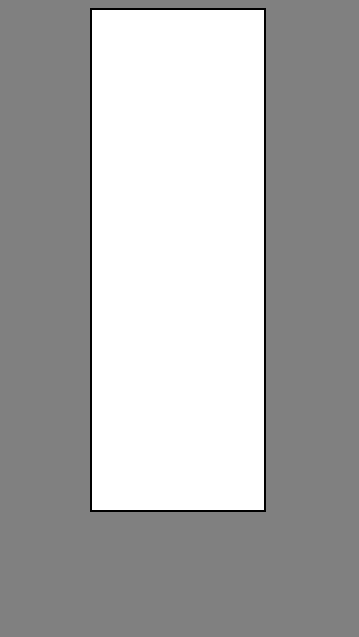
\includegraphics[scale=0.30]{pics/small.png}%
}
\end{figure}
\hspace{1.5cm}Figur 1: Utifrån desktop \hspace{4.8cm} Figur 2: Utifrån mobilen

\newpage

Denna design har endast ett element med egenskaperna:

\vspace{0.5cm}
\begin{verbatim}

div {	
	        margin: 0 auto; //centrerad
	        width:50 %;
	        height:500px;
}

\end{verbatim}

Designen fungerar bra för skrivbordskärmar(bild 1), då rutan är centrerad och symmetrisk. 25\% utrymme på var sida av rutan ger en design som blir läsvänlig och användbart. Däremot är den inte lika optimal när skärmen blir mindre(bild 2). Rutan är fortfarande 50\% av skärmen, vilket gör att  designen blir kompakt i ett utrymme där tanken är att förmedla mycket information på lite plats. 50\% procent av skärmen går till spillo åt utrymme mellan rutan och kanter, vilket får rutan att se ihoptryckt ut. Därav en försämring på design och användbarhet när websidan ses ifrån en mobil.

Med media anrop i CSSen, kallat för media queries, tillåter vi att värden hos ”div” elementet skrivs över när bredden på webläsaren underskrider 380px.

\vspace{0.5cm}
\begin{verbatim}
@media all and (max-width: 380px){
       div {
                margin:0;
                width:100%;
       }
}
\end{verbatim}
\vspace{0.5cm}

Med media anropet kommer ”width” och ”margin” skrivas över när skärmstorleken är 380px eller mindre, ”height” förblir detsamma. Utrymmet mellan kanterna och rutan ändras till 0 och bredden till 100%, vilket innebär hela skärmbredden. Detta leder till att sidan får andra design värden när den ses från en mobil och andra enheter där skärmen har som störst 380px i bredd. Det ger en mer optimal lösning i både användbarhets och design perspektiv, då man kan få plats med mer information och det är lättare för en användare att navigera. 

\vspace{0.5cm}
\begin{figure}[h]
\centerline{%

\includegraphics[scale=0.25]{pics/mobilesmall.png}
}
\end{figure}
\centerline{Figur 3: Användning av media queries för att anpassa websidan till mobilen}

På så sätt kan samma CSS-fil låta element ha olika värden på egenskaper utifrån storleken på webbläsaren. Websidan får en bra design på layouten vare sig skärmstorlek och enhet, vilket är syftet med 
responsive web design.

\subsection{Verktyg}

Inom webdesign utveckling används främst verktygen HTML, CSS och javascript, vilket är det verktyg som kommer att användas under implementeringsfasen i examensarbetet.  I kommande sektion av rapporten kommer verktygen att förklaras för att få en bättre förståelse till kod och termer som används.

\subsubsection{HTML}
HTML står för Hypertext Markup Language och är ett format som definierar strukturen och logiken på en websida. HTML beskriver strukturen genom att märka upp olika delar av sidan med hjälp av taggar som beskriver vilken sorts element det är. En webläsare läser av HTML-koden och kan på så sätt rendera sidan med rätt layout.

Det finns olika sorters taggar inom HTML, stycke, rubrik, tabeller, länkar, listor, sektioner är en av dessa. Inom webutveckling har det under senare tid blivit vanligt att man definierar en sida i olika sektioner med element inom dem. 

\vspace{1cm}
\begin{verbatim}
<div> 
          <h1> Mobile-first eller Desktop-first?</h1>
          <p>Frågan en webutvecklare ställer sig inför skapandet av
           en responsiv websida
          </p>
</div>
\end{verbatim}
\vspace{1cm}

I ovanstående HTML-kod har vi definierat en sektion på sidan med <div> taggen, inom den sektionen har vi en rubrik som definieras med taggen <h1> och ett stycke som definieras med taggen <p>. Taggarna i html-koden bildar tillsammans strukturen på sidan, däremot så har inte html-koden någon kontroll över utseendet för taggarna, det sköts av CSS.  

\subsubsection{CSS}
CSS står för Cascading Style Sheets och är ett språk som beskriver utseendet på html-kod.
Med hjälp av CSS-kod kan olika element i html-koden få ett speciellt utseende i form av storlek, färg och position. Det finns olika sätt att definiera css, man kan definiera det direkt i taggen t.ex <p style=”color:blue; width:50px”>Frågan en webutvecklare ställer sig inför skapandet av en responsiv websida</p> vilket kallas för inline-styling. Man kan även i html filen, definiera utseendet i <head> taggen, vilket kallas för internal styling:

\vspace{0.5cm}
\begin{verbatim}
<head>
           <style>
           p {
           color:blue;
           width:50px;
           }
           </style>
</head>
\end{verbatim}
\vspace{0.5cm}

På så sätt säger man att alla <p> taggar i html-koden kommer att ha dessa egenskaper. Sista sättet är att definiera det i en egen css-fil och länka till det från <head> taggen i html-koden, vilket är det vanligaste sättet. 
\vspace{0.3cm}
\begin{verbatim}
<link rel="stylesheet" type="text/css" href="main.css">
\end{verbatim}
\vspace{0.5cm}

I css-kod defineras utseendet av olika taggar, men möjligheten finns att definiera samma tagg med olika utseenden, detta görs med hjälp av klasser och ids. Ett element kan ha olika klasser eller ids och i css-koden kan klasserna defineras med ett utseende, vilket gör att varje tag som delar klassen delar även utseendet:

\vspace{0.3cm}
I html filen:

\begin{verbatim}
<div id=”main-container”>
          <p class=”paragraf”>Mobile-first vs Desktop-first</p>
</div>
\end{verbatim}
\vspace{0.5cm}
I css filen:

\begin{verbatim}
#main-container {
        width:50%;
        background-color:grey;
}

.paragraf{
        font-size: 125%;
        color:black;
}
\end{verbatim}
\vspace{1cm}

Vid dessa tre olika sätt att definiera utseendet visas enligt prioritering, inline-styling kod först, sedan internal och sist external. Anledningen till att man väljer external främst är för att man slipper definiera utseendet flera gånger, allt är samlat i en fil och det går snabbare att ladda sidans utseende. Därmed hålls det ur en webutvecklares synvinkel, en bra struktur, vilket tillåter webutvecklaren att på upprätthålla teknikerna fluid grid, fluid images och på ett enkelt sätt använda sig av media queries vid implementeringen av en webbsida.

\subsubsection{JavaScript}
JavaScript är ett scriptspråk som inom webutveckling främst används för att hantera dynamiska funktioner för beteendet hos en websida, beteenden som skapas från klientsidan. Med JavaScript kan man t.ex. läsa en användarens klick i websidan och utifrån det kalla på funktioner som kan ändra websidans innehåll eller utseende. Eftersom JavaScript är ett skript språk behövs ingen kompilering och koden kan skrivas direkt i html-filen.

För att JavaScript skall fungera korrekt krävs det dock att webbläsaren har stödjer det. I vissa fall har webläsaren den funktionen men har den avstängd. Tidigare har det varit ett problem att mobila webbläsare inte har haft stöd för JavaScript, vilket har lett till att menyer och pop-up fönster inte har fungerat korrekt när man surfar till sidan via mobilen, men tekniken har utvecklats och numera klarar mobila webbläsare av JavaScript. Men fortfarande finns det en del problem i mobila webbläsare när det kommer till mer komplicerade JavaScript funktioner. Vid websidor som har helt separata mobilsidor kan det vara en fördel då man väljer att inte läsa in all JavaScript som behövs, med responsiva web sidor använder man samma websida för varje enhet, vilket leder till att en mobilenhet laddar all JavaScript och gör att websidan svarar långsamt. En webbutvecklare måste ha det i åtanke och redan från början utveckla en hemsidan vars JavaScript inte är för invecklat för mobilsidan.

\subsection{Mobile-first och Desktop-first}
Tekniken för att skapa responsiva sidor existerar, med hjälp av utvecklingen av ovanstående tekniker och verktyg finns i nuläget möjligheten att skapa en websida som beroende på skärmstorlek har olika designlayouts med en och samma kodgrund. Det finns även kunskap om hur man skall gå tillväga för att skapa en responsiv websida, där en utvecklare med formler och riktlinjer kan lära sig att använda fluid grid, fluid images och media queries på bästa sätt. Men vägen till att skapa en responsiv websida är olika.  I bloggar och forum på webben diskuteras flitigt valet av utvecklingsmetod när det kommer till responsiva webplatser och innan implementeringen av websidan är detta en fråga som med stor sannolikhet dyker upp. Utvecklingsmetoderna man diskuterar om är Mobile-first och Desktop first. Mobile-first och Desktop-first är två olika metoder där det responsiva angreppssättet används. Båda strävar efter samma mål men där frågan handlar mestadels om vilken enhet websidan skall anpassas för först. 

\subsubsection{Mobile-first}
Mobile-first metoden bygger på att man skapar en websida anpassad för mobilskärmen först, för att sedan med hjälp av media queries och en flexibel layout renderera elementen på websidan desto större webläsarfönstret blir.  På så sätt är grund layouten designad för en mobil. Mobile-first anses som en rimlig utvecklingsmetod då man tar till hänsyn antalet mobilanvändare och det behov som finns vid navigering och informationsintagelse från mobilskärmar.  Det betyder att innehåll prioriteras då bristen på plats är ett faktum och fokus läggs på de delar som informationsmässigt är de viktigaste. Det behöver inte nödvändigtvis betyda att hänsyn till prioritering och design inte tas när man utvecklar i desktop-first, utan snarare att prioriteringen för mobilskärm sker vid ett tidigare skede i utvecklingen när man använder sig av mobil-first.

Kodmässigt är grunden anpassad för mobilen, det vill säga att media anrop sker när skärmen blir större, där media queries ser till att skriva om värden klasser. 
\vspace{0.5cm}
 \begin{verbatim}
@media all and (min-width: 480px){
        .main {
                margin:0 auto;
                width:50%;
        }
}
\end{verbatim}

\vspace{0.5cm}
I fallet ovan sker ett anrop när bredden på websidan är som minst 480px, som gör att elementen med klassen main får margin och width skrivs över med nya värden. I fall då mobiler inte klarar av att läsa media queries(fotnot), vilket i dagsläget är få, är detta en optimal lösning då grunden redan är skrivet för mobilen, och en läsning av media queries endast kommer att krävas från en desktop vilket de flesta webläsare klarar av.

\subsubsection{Desktop-first}
Desktop-first metoden bygger på att man utvecklar för skrivbordskärmen och därefter rendererar som sidan desto mindre skärmen blir. Det behöver inte nödvändigtvis betyda att skapar en hel sida för desktop som sedan i efterhand designas om till mobil, utan tanken för mobil finns redan från början men implementeringen sker i synnerhet för skrivbordsskärmen först. Websidor som i efterhand skapas till mobilen, brukar innebära en separat mobilsida då refaktoreringen av kod i samband med att förvandla sidan till responsiv kan innebära en del komplikationer.  

Kodmässigt är grunden anpassad för skrivbordsskärmen, det vill säga att media anrop sker när skärmbredden når en minimum gräns, i form av en mobilskärm, där media queries ser till att skriva om valda klasser.


\vspace{0.5cm}
 \begin{verbatim}
@media all and (min-width: 380px){
        .main {
                margin:0 ;
                width:100\%;
        }
}
\end{verbatim}
\vspace{0.5cm}

I fallet ovan sker ett anrop när bredden är som max 380px. Anropet ger margin och width i klassen main nya värden, anpassade till mobilen.  Desktop-first används med tanken att websidan ska ge en upplevelse, och skall nå en design maximum när man den ses från en skrivbordskärm, upplevelsen utifrån en mobilskärm är inte lika högt prioriterad, men bör innebära en funktionell sida med det nödvändigaste funktionalitet.

\subsubsection{Mobile-first eller Desktop-first, vilken ska man välja?}
Utvecklingen av tekniker och verktyg har gjort det möjligt att kunna applicera metoderna vid skapandet av en websida. Kunskapen om metoderna var för sig har med tiden blivit större i samband med utvecklingen av responsive web design. Däremot ställs webutvecklare kring frågan om vilken metod som appliceras bäst till den typen av websida som skall skapas. I dagsläget finns ingen kunskap om hur bra metoderna appliceras i jämförelse med varandra. Det finns tankar och spekulationer, därefter väljs metod utifrån dessa, komplikationer hanteras men dokumenteras inte och till slut har man en fungerande responsiv websida. Eftersom websidan är färdig implementerad finns ingen anledning till att implementera om en fungerande lösning med en annan metod, därav är kunskapen om samma resultat men med en annan lösning liten.

Användningen av mobilt internet ökar och användningen av internet via en dator kommer med stor sannolikhet att bestå. Vilket gör att en grund för val av metod är högst passande, då det redan nu och i framtiden kommer att kräva mer än en webutvecklares tankar nedskrivna i ett blogginlägg för att fatta ett beslut. Båda metoder har sina fördelar samt nackdelar, frågan är när man kan utnyttja dessa bäst, och kan beslutet av val leda till positiva faktorer vilket andra metoden just i den frågan inte hade kunnat göra.    
\newpage

\section{Syfte}
Syftet med arbetet är att kunna hitta riktlinjer till när en specifik metod appliceras som bäst, det vill säga beroende på faktorer kring websidan hitta den metod som tillför det mest optimala lösningen i en situation. Att hitta en metod som fungerar bäst i alla lägen är inte målet, då det har framgått i litteraturstudie att det existera för många olika vinklar som gör det svårt att hitta en specifik faktor hos en metod som avgör beslutet i alla lägen.

Frågeställningar som besvaras i rapporten är:

\begin{enumerate}
	\item I vilka lägen appliceras metoderna bäst
	\item Vad är för- och nackdelarna med Mobile-first?
	\item Vad är för- och nackdelarna med Desktop-first?
\end{enumerate}

Frågeställning nr 1 baseras på miljö, målgrupp och kontext. Syftet med frågeställningen är att kunna utifrån analys hitta situationer där metoderna visar sig vara fördelaktiga under utvecklingsfasen, vilket hade varit svårare att uppnå med ett annat val av metod. Frågeställning nr 2,3 är att kunna lyfta fram de fördelar och nackdelar som finns vid implementation med de två metoderna. Syftet är att hitta ramar för varje metod vilka en läsare kan relatera till med en egen situation och utifrån det använda det som grund vid val av metod. 

\subsection{Avgränsningar}

Arbetet kommer att enbart fokusera på mobile-first och desktop-first, ett mellanläge som existerar för Ipads, tablets, osv. kommer inte att tas med i arbetet. I dagsläget finns även andra lösningar för mobilawebb t.ex Appar, Hybrida Appar, vilka även har en grund till statistiken för mobilanvändare. Jämförelse mellan dessa och responsive web design kommer inte att göras, utan jämförelsen är inom mobilalösningar i form av responsive web design.

Mobile-first kan tolkas olika, det har förekommit tillfällen då tanken för mobil-first har varit prioriterande medan implementeringen ändå har skett för skrivbordsskärmen först, vilket har tolkats som en mobile-first tillvägagångsätt.  Det är inte fallet i arbetet, utan mobil-first beskrivs i arbetet som en tanke och en implementering avsedd för mobilen i först hand och detsamma för desktop-first. Testfallen under implementeringsdelen kommer att bygga på den teorin(se sida).

\newpage

\subsection{Valtech AB}
Examensarbetet kommer att utföras på Valtech AB i Stockholm. Valtech Sverige fokuserar främst på utveckling av användarvänliga hemsidor, webbapplikationer och intranät. Hos Valtech finns erfarna gränssnittsutvecklare som har stött på problem under utvecklingsprocessen i form av ett beslutstagande av tillvägagångssätt. Därför finns det ett behov hos utvecklare på Valtech att ha en grund för vilka faktorer som är viktigast när det gäller att ta ett beslut om metod. En metod som ger den bästa lösningen för en effektiv utveckling av en responsiv webbplats. Gränsnittssutvecklarna besitter på mycket erfarenhet och kunskap, vilket kan samlas i form av intervjuer för att analyseras och sammanfattas utifrån verkliga situationer som förekommer i företag, för framtida syfte.



\end{document}                 % The input file ends with this command.